\subsection{Construction of LIGO}

\hspace{1cm} The idea of a laser interferometer to detect LIGO started in the 1960s, where American scientists like Joseph Weber, Soviet scientists Mikhail Gertsenshtein and Vladislav Pustovoit, merged their ideas of a basic interferometer based on Michelson's interferometer. In 1967, Rainer Weiss affiliated to Massachusetts Institute of Technology (MIT) published his paper on the analysis of usage of interferometer and with the help of military funding he initiated the construction of interferometer prototype, but it couldn't be completed. But in 1968, Kip S. Thorne did extensive research on gravitational waves and their sources at Caltech, then he was convinced that interferometers could successfully detect gravitational wave. Thus finally LIGO was constructed in Hanford, Washington in 1994 and Livingston, Louisiana in 1995. The construction was completed by 1997, under Barish's leadership.  After successful detection of GW150914, in 2017, Rainer Weiss, Kip Thorne and Barry C. Barish who were the frontiers of Gravitational wave detection won the Nobel Prize in Physics. \\
LIGO is constructed in such a way that it can even feel the changes in the weakest fundamental force. Some important parts of this Gigantic detector are:- 

\subsubsection{LIGO arms}

LIGO's arms are placed orthogonal to each other which extends for $4\,km$ into two perpendicular directions. The arms of LIGO are made of cylindrical tubes each $20\,m$ in length, welded together whose diameter is $1.2\,m$. The tube is made of 304L-steel with a thickness of $3\,mm$ \cite{carpenter2000laser}. This particular material has extremely low carbon content making it relatively resistant to corrosion when compared to other. The tubes are evacuated to a pressure of $10^{-10}$ to $10^{-8}\, torr.$ This is to prevent the scattering of laser and also to not allow sound to interfere (as sound cant travel in vacuum). The arm is constantly evacuated by the Ion pumps to maintain the vacuum inside the arms. Initially when LIGO was set-up it took approximately 40 day to fully evacuate the beam tubes, and it was heated to 150\degree C to remove residual gases. \cite{vacuum} 

\begin{figure}[h]
    \centering
    \subfloat[]{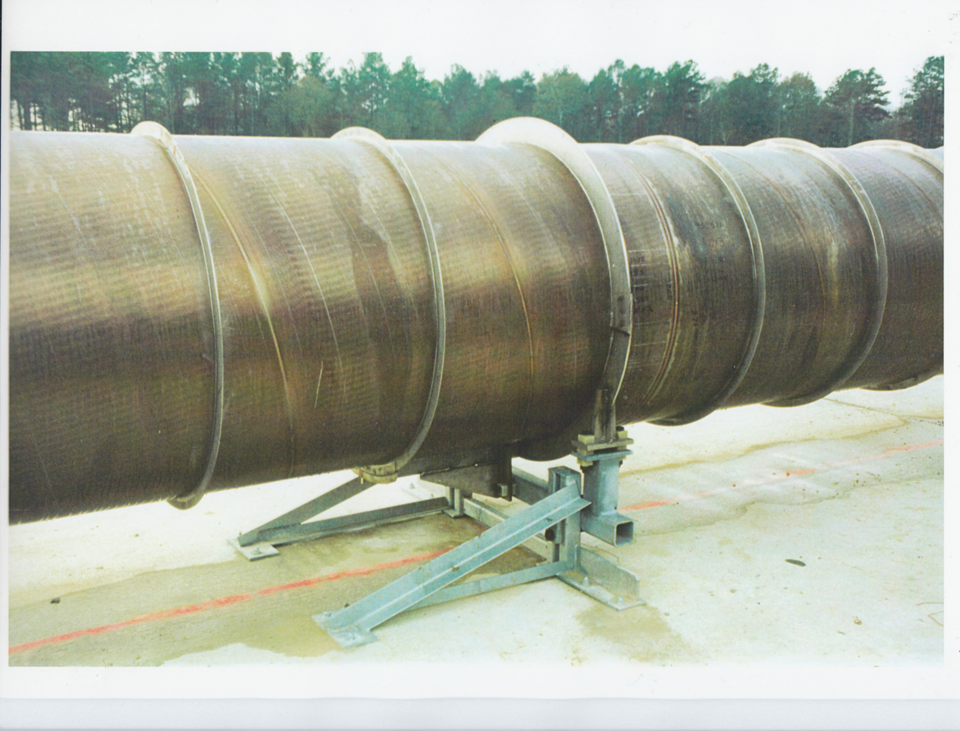
\includegraphics[width = 7 cm, height = 5 cm]{images.tex/BEAM_TUBE_SEGMENT.png}}
    \qquad
    \subfloat[]{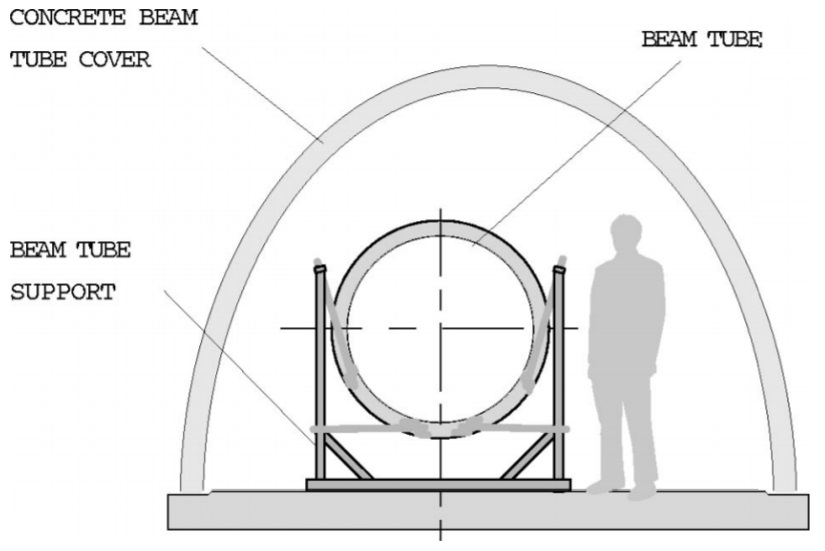
\includegraphics[width = 7 cm, height = 5 cm]{images.tex/C.S view of ligo arm.jpg}}
    \caption{(a) LIGO Beam tube. Source :- \cite{vacuum} (b) C.S view of beam tube. Source:- \cite{althouse2001precision}}
\end{figure}

\subsubsection{Laser system}

The laser used in LIGO has active material to be Nd-YAG (Neodymium - Yttrium Aluminium Garnet) and diode as the pump. Initially the laser output is $4\,W$ and wavelength of lasing light is $808\,nm$ wheich is in near infrared range. This light travels through Non-Planar Ring Oscillator (NPRO), from which a $2\,W$, $1064\,nm$ light called seed beam is generated. This is the laser which will be amplified and begins it's journey in LIGO interferometer. The seed beam is then passed through a Master-Oscillator Power Amplifier (MOPA), which consists of four thin rods of $3\,mm$ thick and $5\,cm$ long which is made similar to glass, using Nd, Y, Li and F$^{-}$. The laser power increases in each of these four rods and finally a 35W laser with the constant wavelength of 1064nm is obtained. It is now further amplified in a High-Power Oscillator (HPO) which is similar to MOPA. This results in an immensely powerful light of 200W. \cite{laser} 

\begin{figure}[h]
    \centering
    \subfloat[]{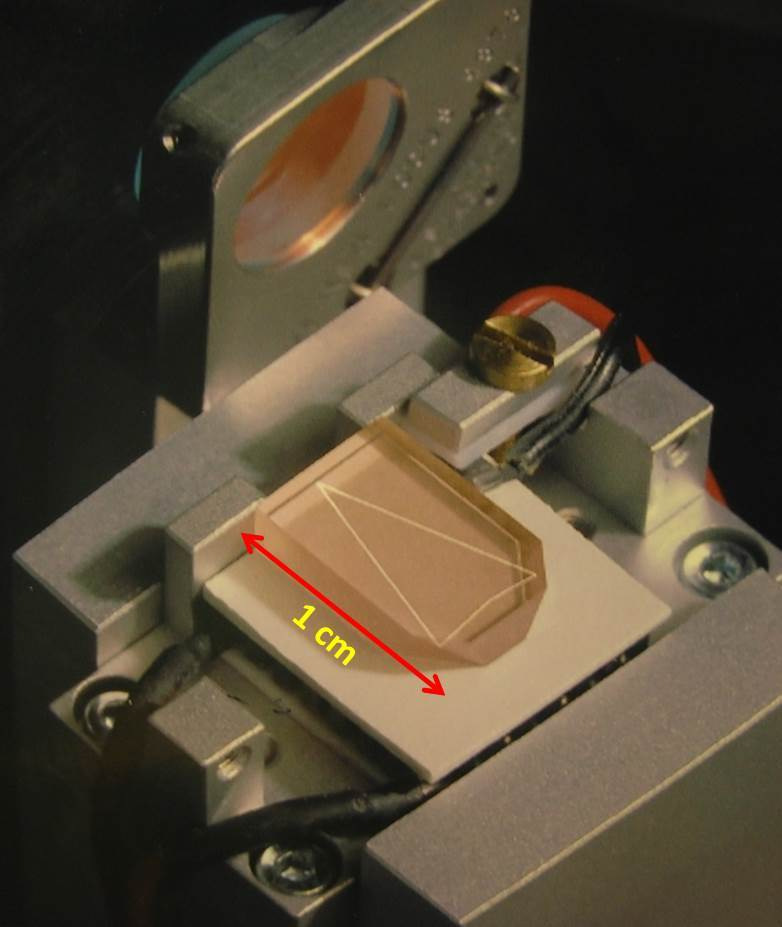
\includegraphics[width = 4.5 cm, height = 5 cm]{images.tex/NPRO.jpg}}
    \qquad
    \subfloat[]{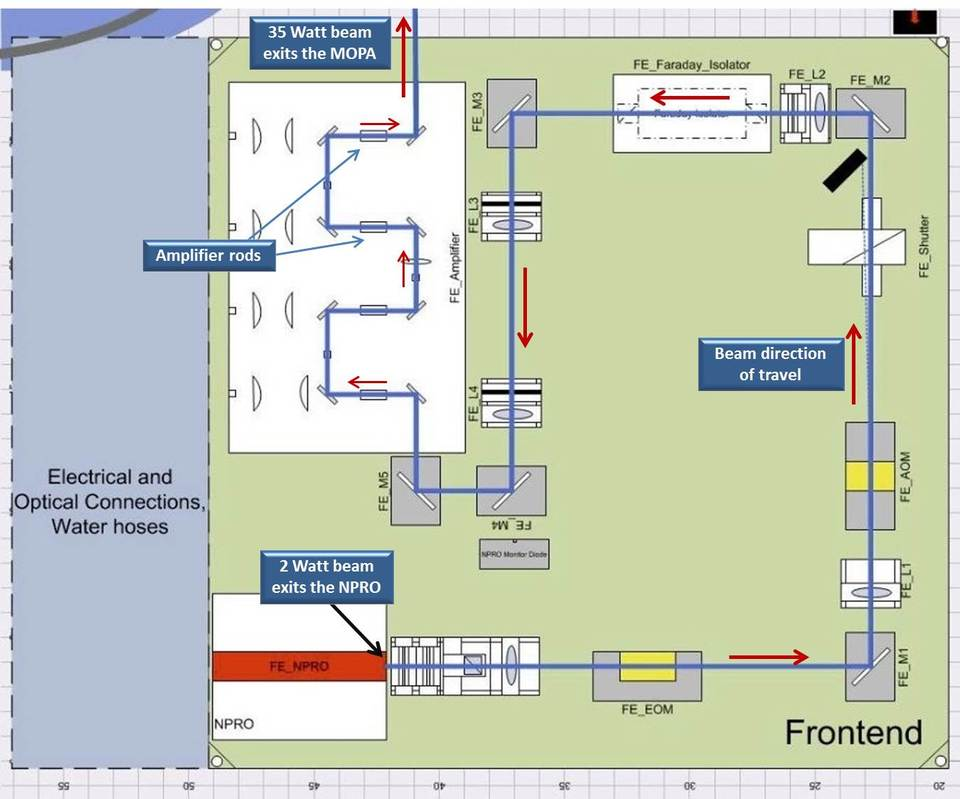
\includegraphics[width = 8.5 cm, height = 5 cm]{images.tex/Laser amplification.jpg}}
    \caption{(a) NPRO crystal. (b) schematic representation of laser amplification. \cite{laser}}
\end{figure}


\subsubsection{Beam Splitter and Mirrors}

Each arm carries two fully reflecting mirrors at its ends and a partially reflecting mirror called as Beam splitter is present at the common vertex of the arms. The space between the mirrors forms Fabry-Perot cavity. The light travels 4$km$ from one end to other, but this cavity makes the laser light to reflect approximately 300 times, so apparently the laser travels a total of $1200\,km$, this increases the laser power to $750\, kW$. The mirrors are coated extensively to nanometer smoothness (i.e the imperfections on the surface of mirror is in the order of nanometers). This is required to make the system so precise to detect even very feeble GWs. \cite{mirrors}

\begin{figure}[h]
    \centering
    \subfloat[]{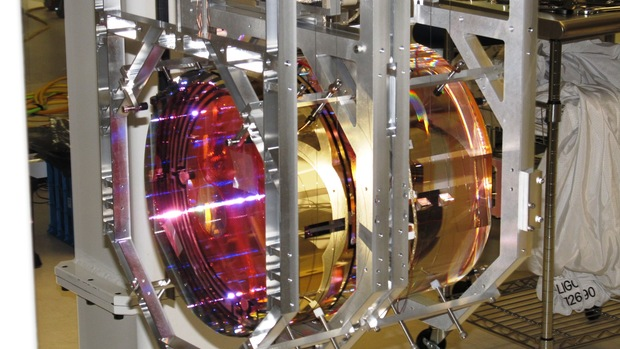
\includegraphics[width = 7 cm, height = 5 cm]{images.tex/LIGO_mirror.jpeg}}
    \qquad
    \subfloat[]{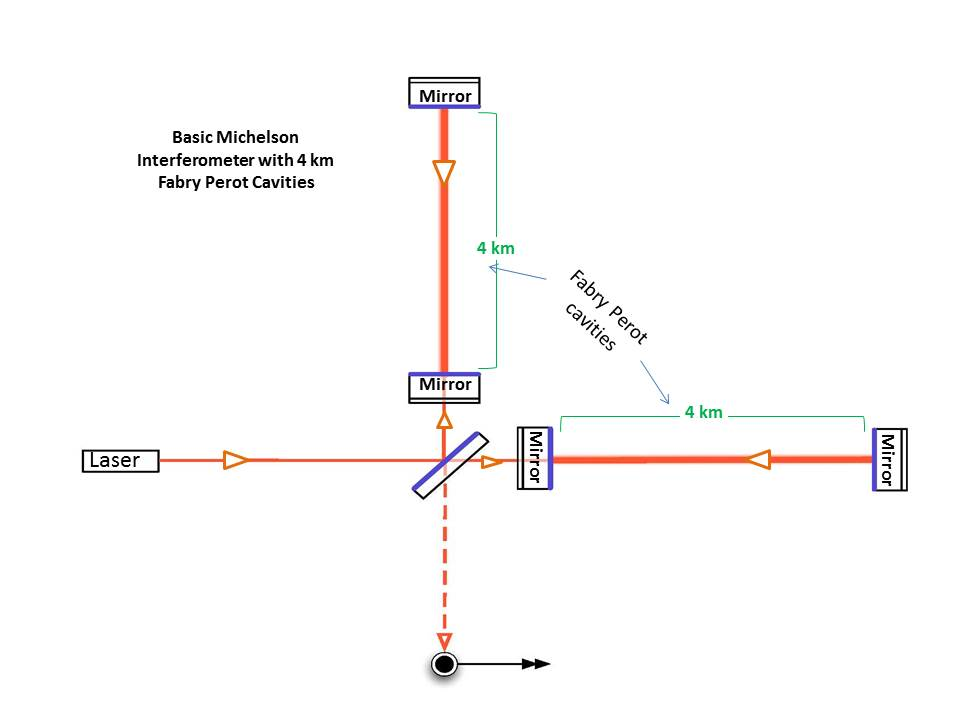
\includegraphics[width = 7 cm, height = 5.5 cm]{images.tex/Fabry Perot cavity.jpg}}
    \caption{(a) Fully reflecting mirror.\cite{mirrors} (b) Fabry-Perot cavity. \href{https://www.ligo.caltech.edu/page/ligos-ifo}{Source}}
\end{figure}


\subsubsection{Test mass and Photo-detector}

The fully reflecting mirrors are $40 \,kg$ each with thickness of $20\,cm$ and width of $34\,cm$. They act as test masses and are at 4 kilometers away from each other. This test mass is one among three other mass which are hung to a quadruple suspension system aided by silica fibers. They reduce the effect of noise vibration by 100 million times by the time it reaches the mirrors. This acts as a passive seismic isolation system. \cite{mirrors} Then finally the last component is the photo detector. Since the wavelength of operational laser is $1064\,nm$, which lies in infrared spectrum, the photo detector should work in the infrared region. LIGO uses Broad Band Photo Detector (BBPD) which is built around a low capacitive, series resistant silicon photo-diode "FFD-100", and coupled to a $50\,\Omega$  Radio frequency amplifier called Teledyne Cougar AP389. \cite{BBPD}

\pagebreak
